%------------3.1--------------------------------------%
\section{Pipeline}
\label{whole_pipeline_intro}

\begin{figure}[h]
    \centering
    % \hspace*{-8mm}
    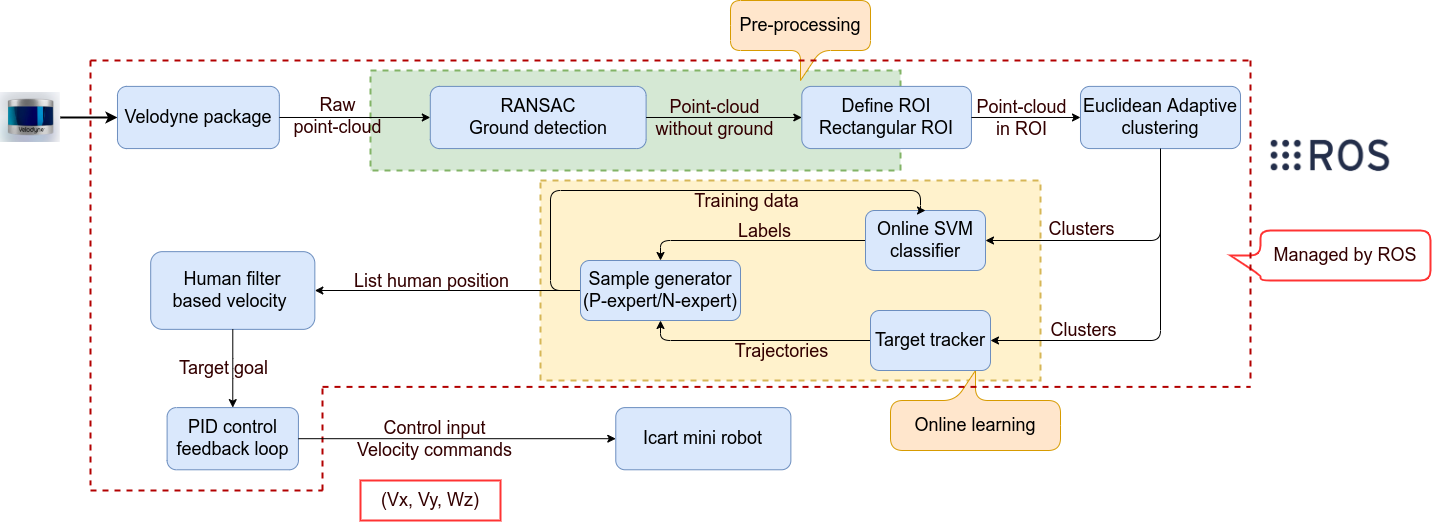
\includegraphics[width=1.0\linewidth]{figures/chap3_fig/pipeline.png}
    \caption{A Pipeline of the ROS-based Human Following Robot system}
    \label{Chap3:Fig1}
\end{figure}

% This section generalizes the proposed pipeline, which is the heart of this thesis.
This section describes the proposed pipeline, which is the heart of this thesis.
This pipeline takes point cloud obtained from a 3D LiDAR onboard an mobile robot as an input
and outputs the final velocity commands for the mobile robot to follow the identified human effectively in
an indoor environment. This pipeline is illustrated as a block diagram in Figure \ref{Chap3:Fig1} above.
The whole process is utterly managed and coded in ROS (Robot Operating System) framework \cite{ros_original}.
In principle, the pipeline can be split into 4 main stages, which are pre-processing step, clustering step,
classification step and control step. The pre-processing step contains RANSAC ground extraction and ROI(Region of Interest) definition,
which is presented in section \ref{pre-processing_step_section}. The clustering step uses Euclidean Adaptive clustering method and is depicted
in section \ref{Euclidean_cluster_section}. Then, section \ref{online_learning_section} describes online learning for SVM(Support Vector Machine) which is the human classification
step. Finally, the control phase is discussed in section \ref{pid_section}, which comprises 2 smaller modules: human filter-based velocity
and PID control feedback loop. The whole pipeline is written in C++ and maintained in author's Github repository.

%------------3.2--------------------------------------%
\section{Pipeline breakdown and details}

%------------3.2.1--------------------------------------%
\subsection{LiDAR point cloud pre-processing step}
\label{pre-processing_step_section}

In this pre-processing step, the ground plane is extracted and removed from the
raw point cloud of Velodyne LiDAR using RANSAC algorithm. RANSAC \cite{ransac} stands for Random Sample
Consensus, which is considered to be a congruous technique to detect and filter out any inliers point cloud
in any set of point clouds using some pre-defined models such as plane model or circle model. RANSAC algorithm used to detect
the plane model is shown in the Algorithm \ref{Chap3:Alg1}. First, the algorithm will select any 3 points in the space randomly to form
a plane. Then, the we evaluate the plane model coefficients $a,b,c,d$ that contains those previous selected points.


\begin{algorithm}[h]
    \caption{RANSAC(Random Sample Consensus) ground plane detection algorithm  \cite{ransac}}
    \label{Chap3:Alg1}
    \begin{algorithmic}[1]
        \Ensure Point cloud data $P^*$ of the plane model
        \Require Point cloud data $P$, where $p_i=[x,y,z] \in P$;
        \State Randomly select three non-collinear unique points $\{p_i, p_j, p_k\}$ from $P$;
        \State Compute the model coefficients from the three points $(ax + by + cz + d = 0)$;
        \State Compute the distances from all $p \in P^* \subset P$ to the plane model $(a,b,c,d)$;
        \State Count the number of points $p^* \in P$ whose distance $d$ to the plane model falls between $0 \leq |d| \leq |d_t|$, where $d_t$ represents a user specified threshold.
    \end{algorithmic}
\end{algorithm}

% \begin{figure}[h]
%     \centering
%     % \hspace*{-8mm}
%     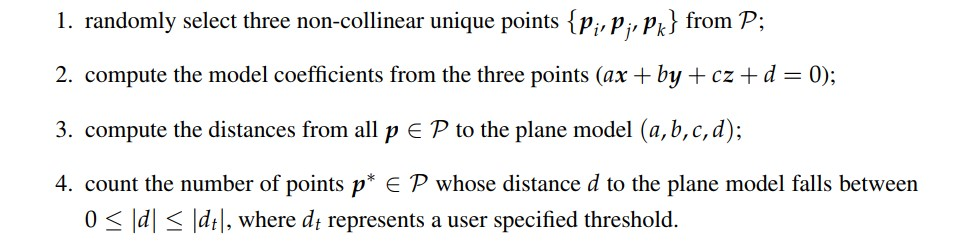
\includegraphics[width=1.0\linewidth]{figures/chap3_fig/preprocess/ransac_algorithm.jpg}
%     \caption{RANSAC(Random Sample Consensus) ground plane detection algorithm \cite{ransac}}
%     \label{Chap3:Fig2}
% \end{figure}


Next, distance from all remaining points is calculated to that plane model, as visualised in Figure \ref{Chap3:Fig3}. A distance
threshold will be set manually and the total number of points whose distances fall within this range will be recorded in each iteration.
This process will be looped until the maximum number of points is reached. For a set of 3D point clouds, especially point clouds captured
in indoor environment such as corridor or in the building, there is a large number of points that will belong to the ground. If those
point clouds are extracted from the set, the next analysis step will be much faster since the computational
time is greatly reduced. Also, filtering out ground point clouds can make the classification step for all points above the ground
plane easier. An example of RANSAC application to extract ground point clouds is shown in Figure \ref{Chap3:Fig4}. When applying
RANSAC, it is assumed that the ground in the experimental environment is completely flat and not rough.

\begin{figure}[h]
    \centering
    % \hspace*{-8mm}
    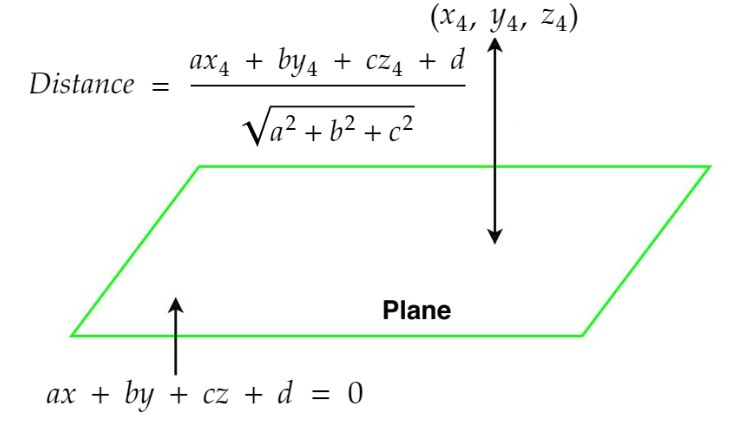
\includegraphics[scale=0.6]{figures/chap3_fig/preprocess/ransac_plane.jpg}
    \caption{RANSAC plane distance estimation \cite{ransac_1}}
    \label{Chap3:Fig3}
\end{figure}

% \clearpage

\begin{figure}[h]
    \centering
    % \hspace*{-8mm}
    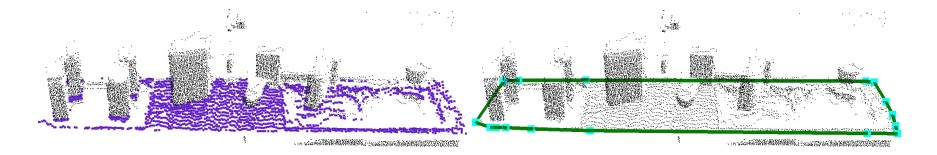
\includegraphics[width=1.0\linewidth,scale=0.8]{figures/chap3_fig/preprocess/ransac_example.jpg}
    \caption{Example of resultant inliers (purple) point support best planar model (ground)  \cite{rusu_thesis}}
    \label{Chap3:Fig4}
\end{figure}

After performing ground segmentation, we need one more small step to accomplish this pre-processing step. Point cloud obtained from
LiDAR scan, after being removed ground points, will be simplified by creating a region of interest(ROI). To put it
differently, we will trim these remaining point cloud by making a box around the mobile robot and get rid of all points outside
this boudary box\cite{cnn_uav}. Robot attached with LiDAR sensor will be the center of this box and in this research, the dimensions
of this box is 10 x 10 x 2m because we want to observe full body of human.


%------------3.2.2--------------------------------------%
\subsection{Adaptive Euclidean clustering}
\label{Euclidean_cluster_section}

In this step,  point cloud that is above the ground and inside a boundary box will be clustered into multiple
separated objects, like the example in Figure \ref{Chap3:Fig5}. This clustering method is known as Euclidean
object clustering technique \cite{rusu_thesis,cnn_uav} and its pseudocode is shown in Algorithm \ref{Chap3:Alg2}.
This method is also regarded as prevalent 3D point cloud analysis technique \cite{3d_pc_analysis}.
This algorithm takes point cloud data P as an input and outputs an array of point cloud clusters C. These
clusters can contain both human and non-human objects that will be fed to the next classification stage.
To implement this algorithm, first kd-tree representation \cite{rusu_thesis} will be created. Array of clusters
C and small set of points Q will be first inilialised, then we will jump into the main loop of Euclidean clustering
method. Point $p_i$ will be added to Q in sequence and in each iteration, another loop is made to search
for any point ${p_i}^k$ within a sphere of radius $r$. This radius is smaller than an assigned threshold
$d^*$. This nested loop will compile until all suitable points are added to Q and Q is added to C. This algorithm
will terminate if all point cloud have been clustered.



\begin{figure}[h]
    \centering
    % \hspace*{-8mm}
    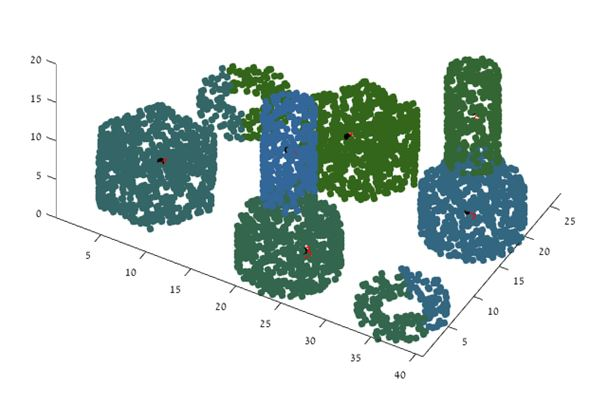
\includegraphics[scale=0.5]{figures/chap3_fig/euclidean/euclidean_example.jpg}
    \caption{Example of Euclidean object clustering  \cite{rusu_thesis}}
    \label{Chap3:Fig5}
\end{figure}

% \begin{figure}[h]
%     \centering
%     % \hspace*{-8mm}
%     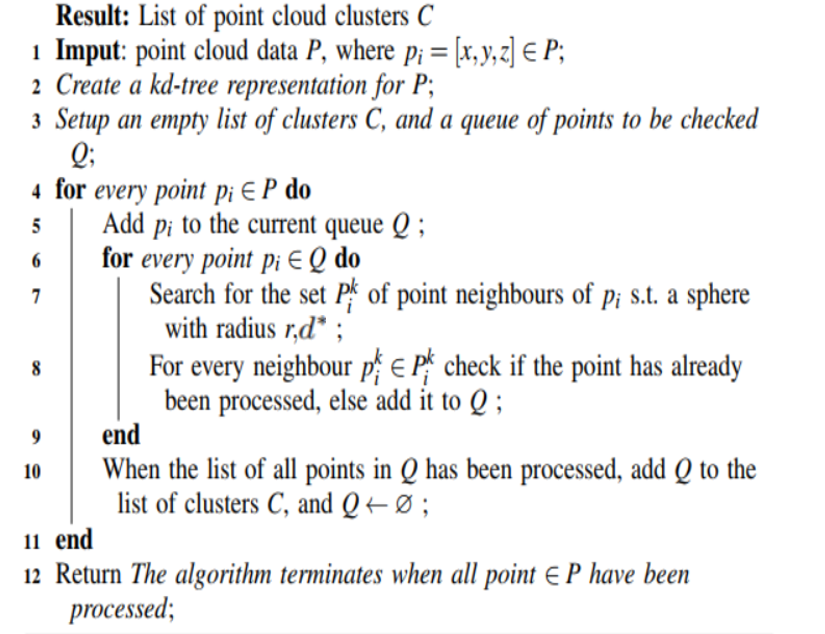
\includegraphics[width=1.0\linewidth]{figures/chap3_fig/euclidean/euclidean_cluster_algorithm.png}
%     \caption{Euclidean clustering algorithm  \cite{rusu_thesis,cnn_uav}}
%     \label{Chap3:Fig6}
% \end{figure}

\begin{algorithm}[h]
    \caption{Euclidean clustering algorithm  \cite{rusu_thesis,cnn_uav}}
    \label{Chap3:Alg2}
    \begin{algorithmic}[1]
        \Ensure List of point cloud clusters C
        \Require Point cloud data $P$, where $p_i=[x,y,z] \in P$;
        \State Create a Kd-tree representation for $P$;
        \State Setup an empty list of clusters $C$, and a queue of points to be checked $Q$;
        \For{every point $p_i \in P$}
        \State Add $p_i$ to the current queue $Q$;
        \For {every point $p_i \in Q$}
        \State Search for the set ${p_i}^k$ of point neighbours of $p_i$ s.t a sphere with radius $r,d^*$
        \State For every neighbour ${p_i}^k \in {p_i}^k$ check if the point has already been processed, else add it to Q;
        \EndFor
        \State When the list of all points in $Q$ has been processed, add $Q$ to the list of clusters $C$, and $Q \gets \emptyset$
        \EndFor
        \State Return the algorithm terminates when all point $\in P$ have been processed;
    \end{algorithmic}
\end{algorithm}

However, although Euclidean algorithm is fast and robust, it has one large disadvantage
that should be taken into account. The hindrance of this method lies in the threshold
$d^*$ parameter. In fact, the accuracy of the clustering result depends predominantly on the the threshold
value. As can be observed in Figure \ref{Chap3:Fig7}, if $d^*$ is too large, point cloud obtained
from some objects can be clustered together. On the contrary, small $d^*$ leads to the consequence
that single target can be divided into multiple clusters. Also, according to \cite{online_learning}, the
human form generated by LiDAR scan varies enormously with respect to the distance between human and LiDAR sensor, as
shown in Figure \ref{Chap3:Fig8} because of LiDAR vertical angular resolution. Thus, we will
tune this threshold value using the scan range of LiDAR \cite{online_learning} using this equation below:

\begin{equation}
    \label{Chap3:Eq1}
    d^* = 2r \tan \frac{\theta}{2}
\end{equation}

In equation \ref{Chap3:Eq1}, r denotes the detected range of LiDAR and $\theta$ is the LiDAR vertical
angle resolution respectively.

\begin{figure}[h]
    \centering
    % \hspace*{-8mm}
    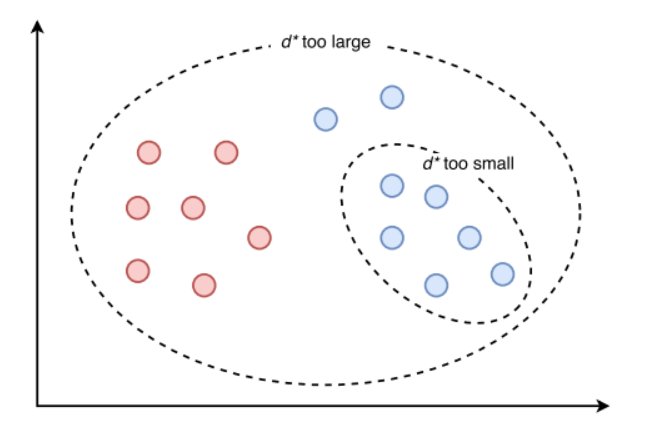
\includegraphics[scale=0.5]{figures/chap3_fig/euclidean/3_2_1.png}
    \caption{Different $d^*$ lead to different clustering results  \cite{online_learning,online_learning_2020}}
    \label{Chap3:Fig7}
\end{figure}

\begin{figure}[h]
    \centering
    % \hspace*{-8mm}
    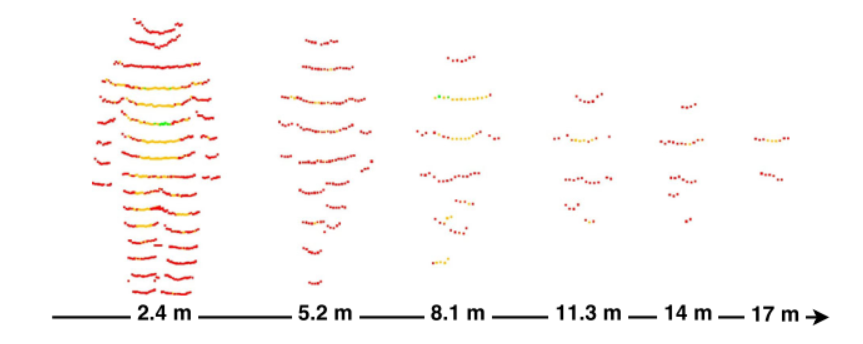
\includegraphics[width=1.0\linewidth]{figures/chap3_fig/euclidean/3_2_2.png}
    \caption{Shape of human point clouds with respect to distance from LiDAR  \cite{online_learning,online_learning_2020}}
    \label{Chap3:Fig8}
\end{figure}

Accordingly for different detection range of LiDAR, an appropriate threshold value
will be determined to make the final clustering result more precise compared to the
traditional Euclidean method. The result of this clustering step will be shown in section
\ref{cluster_result} in Chapter \ref{Chap:ExperimentSetup_Results} below.

% \begin{figure}[h]
%     \centering
%     % \hspace*{-8mm}
%     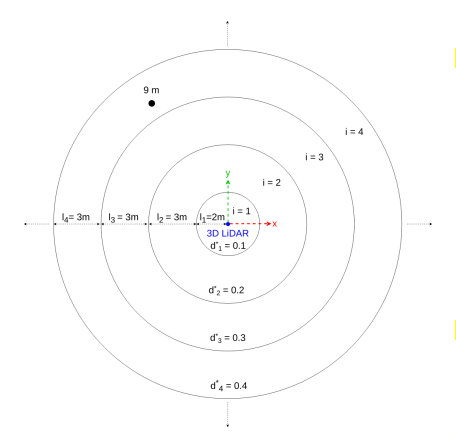
\includegraphics[scale = 1.0]{figures/chap3_fig/euclidean/3_2_3.png}
%     \caption{Values of $d^*$ for various regions \cite{online_learning_2020,online_learning}}
%     \label{Chap3:Fig9}
% \end{figure}

% \begin{figure}[h]
%     \centering
%     % \hspace*{-8mm}
%     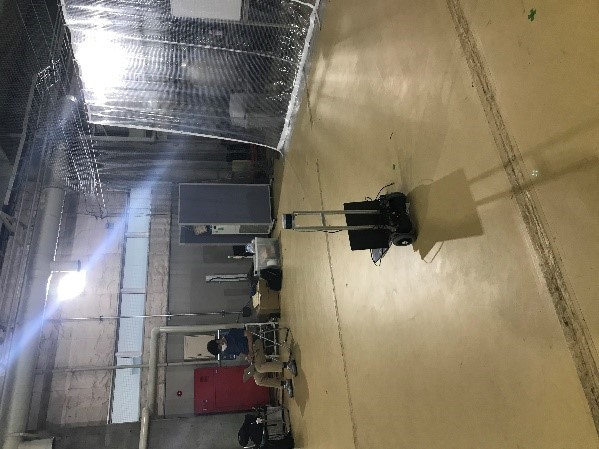
\includegraphics[width=1.0\linewidth,angle = -90]{figures/chap3_fig/euclidean/3_2_4.jpg}
%     \caption{Testing hall}
%     \label{Chap3:Fig10}
% \end{figure}

% \begin{figure}[h]
%     \centering
%     % \hspace*{-8mm}
%     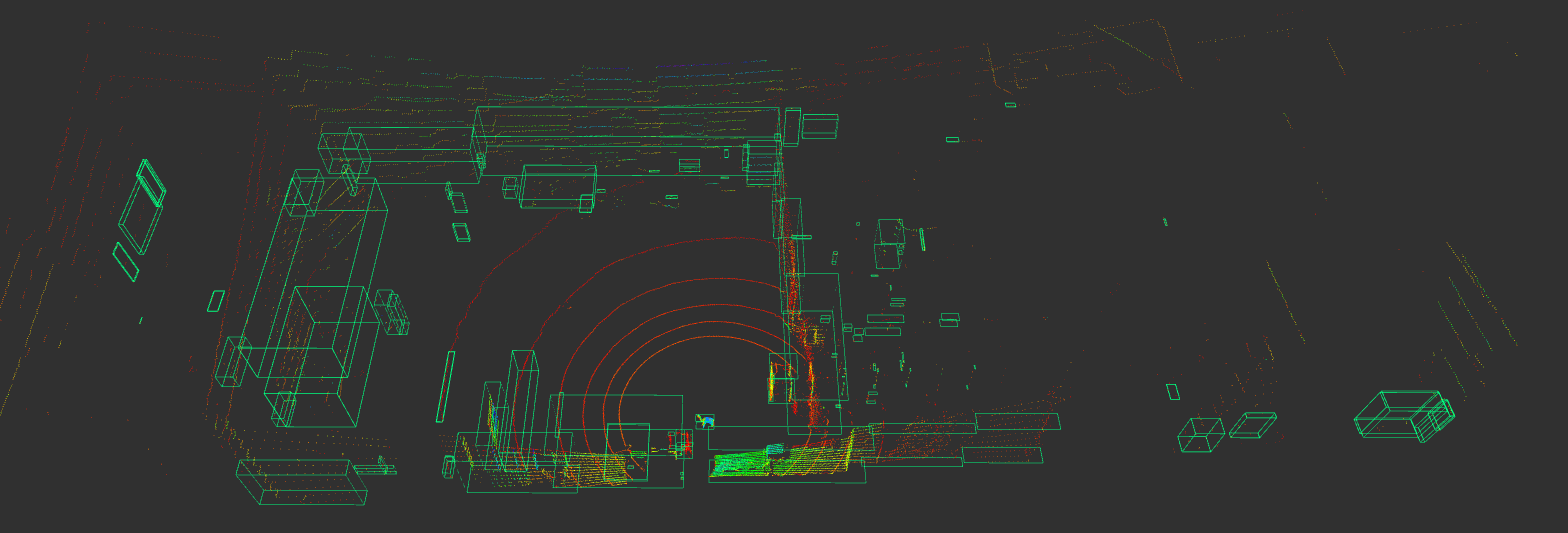
\includegraphics[width=1.0\linewidth]{figures/chap3_fig/euclidean/3_2_5.png}
%     \caption{Testing hall result}
%     \label{Chap3:Fig11}
% \end{figure}

% \begin{figure}[h]
%     \centering
%     % \hspace*{-8mm}
%     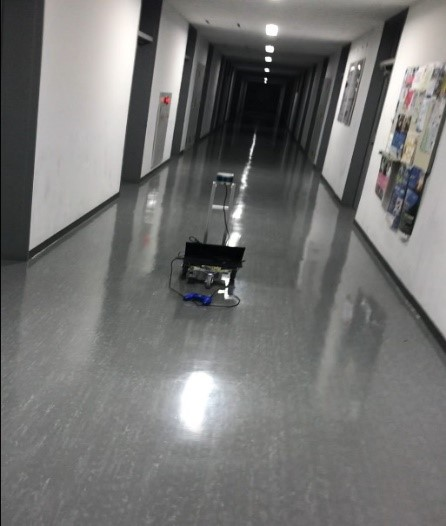
\includegraphics[width=1.0\linewidth]{figures/chap3_fig/euclidean/3_2_6.jpg}
%     \caption{Corridor environment}
%     \label{Chap3:Fig12}
% \end{figure}


% \begin{figure}[h]
%     \centering
%     % \hspace*{-8mm}
%     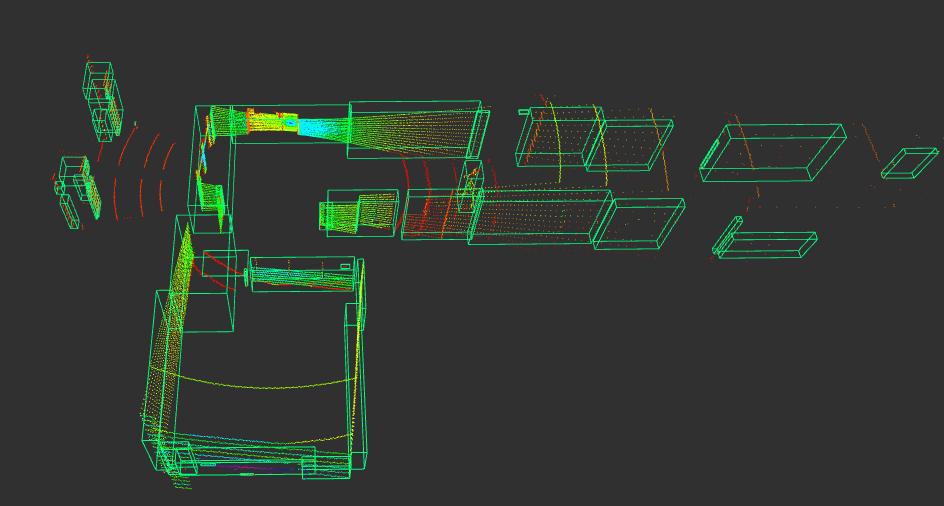
\includegraphics[width=1.0\linewidth]{figures/chap3_fig/euclidean/3_2_7.png}
%     \caption{Corridor environment test}
%     \label{Chap3:Fig13}
% \end{figure}


%------------3.2.3--------------------------------------%
\subsection{Online learning for SVM human classification }
\label{online_learning_section}

The online learning for SVM human classification method which is the most crucial
component of the entire system will be described and analyzed in this section. Figure
\ref{Chap3:Fig14} shows the framework of this learning framework. In short, online learning
process can be broken into 3 parts: the multi-target tracker, human SVM classifier and
P-N sample generator \cite{online_learning}.


\begin{figure}[h]
    \centering
    % \hspace*{-8mm}
    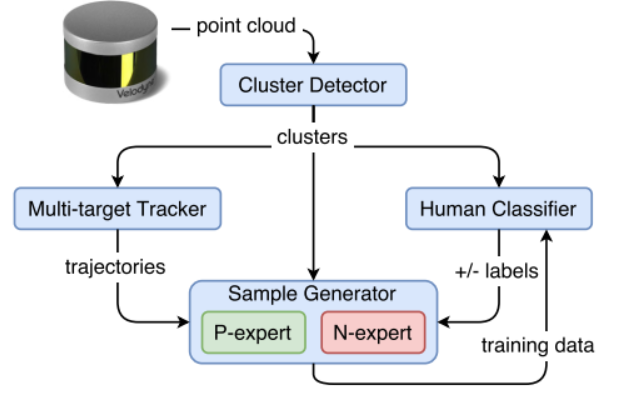
\includegraphics[scale=0.6]{figures/chap3_fig/onlineSVM/3_3_1.png}
    \caption{Online learning framework \cite{online_learning_2020}}
    \label{Chap3:Fig14}
\end{figure}

Each of these part has its own task to complete this online process. The tracker component
estimates the position of each cluster in real time and yields all cluster's trajectories.
Concurrently, the classifier will do its work - classifies whether the cluster is human or
non-human based on the model trained by SVM method. However, the model is not static, it will
be updated continuously with the support from the sample generator. This sample generator
will be the judge in this scenario. In specific, it will correct positive and negative
samples by employing clusters' trajectories information obtained from the tracker and produces
new training data for SVM algorithm. The classifier will be retrained again until some terminating
conditions are satisfied.

The procedure briefly described above is eminently propitious when handling datasets which
are intricate to gather such as human 3D point cloud dataset. Human often has various poses
and different characteristics such as height, body thickness and so on. For that reason, collecting
human datasets for training is considered as tough work and normally requires much efforts to make
good datasets. However, since some features such as point cloud's reflection intensity are completely
distinct, using open-source dataset which is already available on the Internet, namely KITTI is
not appropriate. Thus, batch-incremental training \cite{online_learning,online_learning_2020} as in
Figure \ref{Chap3:Fig14} is effective because new human data is collected online when conducting the
experiment.

EKF (Extended Kalman Filter) and NN(Nearest neighbor) data association \cite{online_learning,online_learning_2020,probab_robot}
are utilised for the cluster tracking process. Although the data obtained is three-dimensional,
only 2D data (i.e x and y coordinates) is used for the tracking. So in this tracking algorithm,
human is supposed to move on a flat plane which should be correct in most indoor environment.
To use EKF, 2 models including velocity model and obseravtion model will be built. The method is much similar
to the traditional Kalman filter, the only difference here is to first linearise all models.
Once the cluster is detected and observed, new cluster states are updated using the polar obseravtion model.
NN data association will be exploited to operate several perceived clusters simultaneously so that all EKFs are
updated in synchronicity \cite{online_learning,online_learning_2020}.

LIBSVM \cite{libsvm} is used to implement the human classifier part of the framework. For this classification task, each human training data has one label and 62 features. The class label can be either 1 (human)
or -1(non-human) and all features using to train the human SVM model are shown in Table \ref{Chap3:Table1} below. The purpose
of SVM is to generate a model that can predict the label of input data, to classify whether this cluster is human or not using
only cluster's features information. We add one more feature $f_3$ or cluster volume, compared to 61 features in \cite{online_learning}.

\begin{table}[h!]
    \centering
    \begin{tabular}{||c|c|c||}
        \hline
        \rowcolor{lightgray}
        \textbf{Feature} & \textbf{Description}                                & \textbf{Dimension} \\ [0.5ex]
        \hline\hline
        $f_1$            & Number of points in cluster                         & 1                  \\
        $f_2$            & Minimum cluster distance from LiDAR                 & 1                  \\
        $f_3$            & Cluster volume                                      & 1                  \\
        $f_4$            & 3D covariance matrix of cluster                     & 6                  \\
        $f_5$            & Normalized moment of inertia tensor                 & 6                  \\
        $f_6$            & Slice feature of the cluster                        & 20                 \\
        $f_7$            & Reflection intensity's distribution (mean, std dev) & 27                 \\ [0.5ex]
        \hline
    \end{tabular}
    \caption{All features for human classification}
    \label{Chap3:Table1}
\end{table}

In this step, C-SVC (C-Support Vector Classification) of LIBSVM is used. The mathematical concept of C-SVC is
constructed as in \cite{libsvm,guide_svm}. For $x_i \in {\mathbb{R}}^{n}$ and output label vector $y_i \in \{ 1,-1 \}$,
C-SVC optimizes this problem:

\begin{equation}
    \label{Chap3:Eq2}
    \begin{split}
        \min_{\alpha}\quad & \frac{1}{2}{\alpha}^{T}Q \alpha - e^T\alpha \\
        \text{subject to } \quad & y^T \alpha = 0 \\
        \text{with } \quad &  0 \leq {\alpha}_i \leq C, i = \{ 1,2,..,62\}
    \end{split}
\end{equation}

% \begin{align*}
%     \min_{\alpha}\quad      & \frac{1}{2}{\alpha}^{T}Q \alpha - e^T\alpha \\
%     \text{subject to }\quad & y^T \alpha = 0                              \\
%     \text{with }  \quad     & 0 \leq {\alpha}_i \leq C, i = \{ 1,2 \}
% \end{align*}

In equation \ref{Chap3:Eq2}, $e$ is vector of all 1 and Q is 62x62 matrix with
$Q_{ij} = y_i y_j K(x_i,x_j)$ . K is defined as kernel function with  $K(x_i,y_j) = {\phi (x_i)}^T \phi (x_j)$ \cite{libsvm,guide_svm}.
There are several kernel functions has been defined such as linear, polynomoial, radial basis function (RBF)
and sigmoid. Among of them, \cite{guide_svm} proposed that RBF kernel should be used. Thus, in
this research, the following kernel function will be used:

\begin{equation}
    K(x_i,y_j) = e^{- \gamma {\|x_i -y_j \|}^2}
\end{equation}

where $C$ and $\gamma$ are 2 parameters which are tuned beforehand.

The sample generator in Figure \ref{Chap3:Fig14} consists P-expert and N-expert. The relation between testing and
real human data is shown in Figure \ref{Chap3:Fig16} below.

% \begin{figure}[h]
%     \centering
%     % \hspace*{-8mm}
%     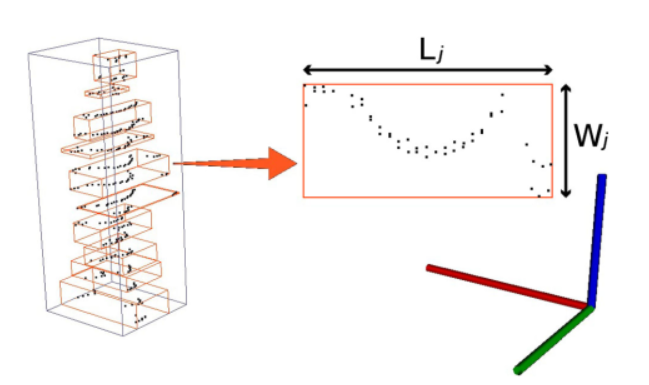
\includegraphics[width=1.0\linewidth]{figures/chap3_fig/onlineSVM/3_3_2.png}
%     \caption{Example of the slice feature \cite{kidono,online_learning_2020}}
%     \label{Chap3:Fig15}
% \end{figure}

\begin{figure}[h]
    \centering
    % \hspace*{-8mm}
    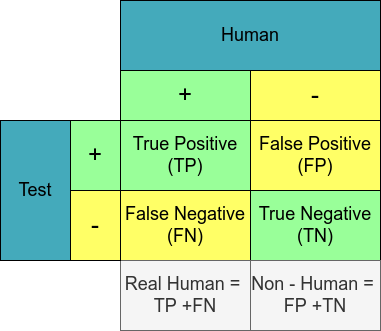
\includegraphics[scale=0.7]{figures/chap3_fig/onlineSVM/TN_FN.png}
    \caption{Positive and Negative clusters}
    \label{Chap3:Fig16}
\end{figure}

From Figure \ref{Chap3:Fig16}, real human clusters are defined as the sum of TP (True Positive) samples and
FN (False Negative) while non-human clusters are the total of FP(False Positive) and TN(True Negative). Evidently,
FN and FP are only 2 cases that must be reduced if we want better classification accuracy. That is where the role of
the sample generator takes place. In specific, all clusters which are categorised as negative samples
are fed to the P-expert of the generator, then this P-expert will assess FN samples and renovate them to positive samples.
Similarly, all clusters which are considered as postive samples in the initial training are fed to the
N-expert and only FP will be transform into negative samples.  This new augmented training data will be
exploited to retrain the whole human classifier \cite{online_learning}. The way P-expert and N-expert
filters out FN and FP samples respectively is genuinely simple. P-expert relies on human-like
trajectory whereas N-expert is governed by approximate static objects. In short, there will be some variances conditions
that have to be satisfied to be considered whether is is human-like or static samples \cite{online_learning}. The
training result will be shown in section \ref{online_svm_result}.



% \textcolor{red}{
% Fig.~\ref{Chap3:Fig16} is too big.
% How you make figures? Vector style figures are preferable more than bitmap ones.
% }


% \begin{figure}[h]
%     \centering
%     % \hspace*{-8mm}
%     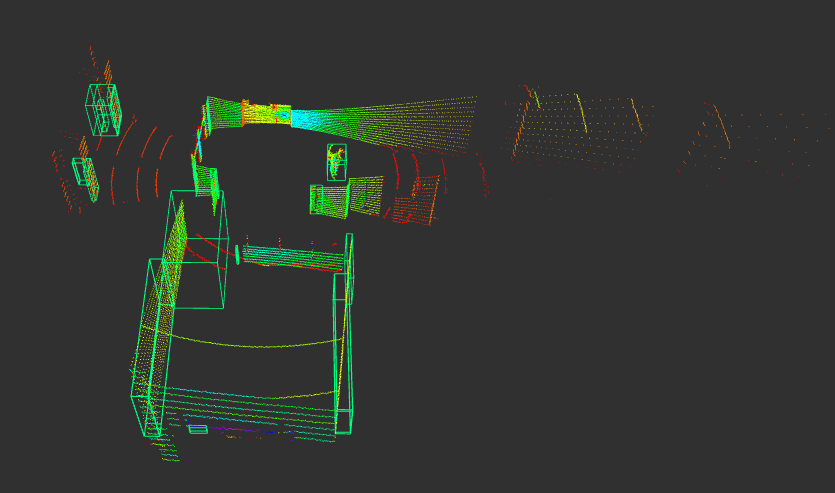
\includegraphics[width=1.0\linewidth]{figures/chap3_fig/onlineSVM/online_train_round1.png}
%     \caption{Online train round 1 (initial)}
%     \label{Chap3:Fig17}
% \end{figure}

% \begin{figure}[h]
%     \centering
%     % \hspace*{-8mm}
%     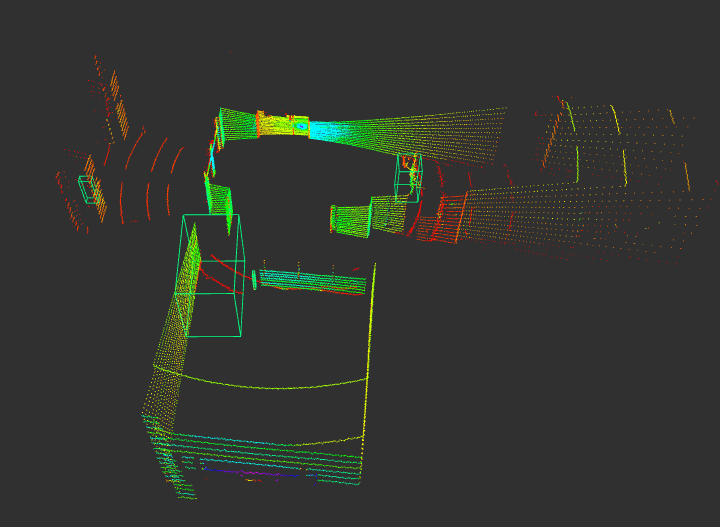
\includegraphics[width=1.0\linewidth]{figures/chap3_fig/onlineSVM/online_train_round3.png}
%     \caption{Online train round 3}
%     \label{Chap3:Fig18}
% \end{figure}

% \begin{figure}[h]
%     \centering
%     % \hspace*{-8mm}
%     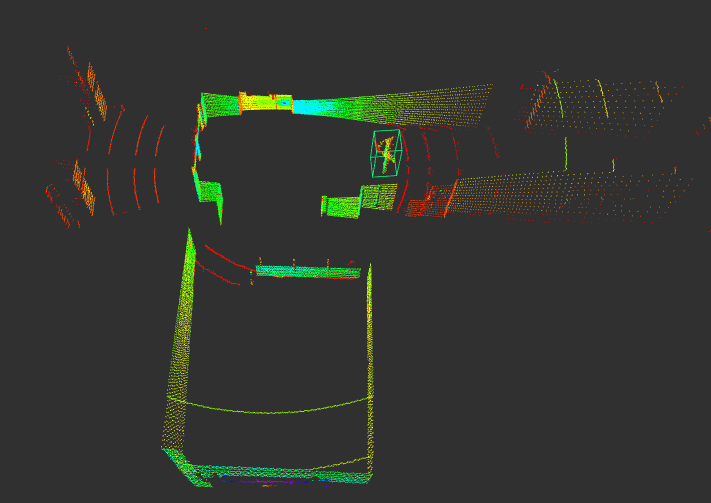
\includegraphics[width=1.0\linewidth]{figures/chap3_fig/onlineSVM/online_train_round5.png}
%     \caption{Online train round 5}
%     \label{Chap3:Fig19}
% \end{figure}

% \begin{figure}[h]
%     \centering
%     \begin{subfigure}{.5\linewidth}
%       \centering
%       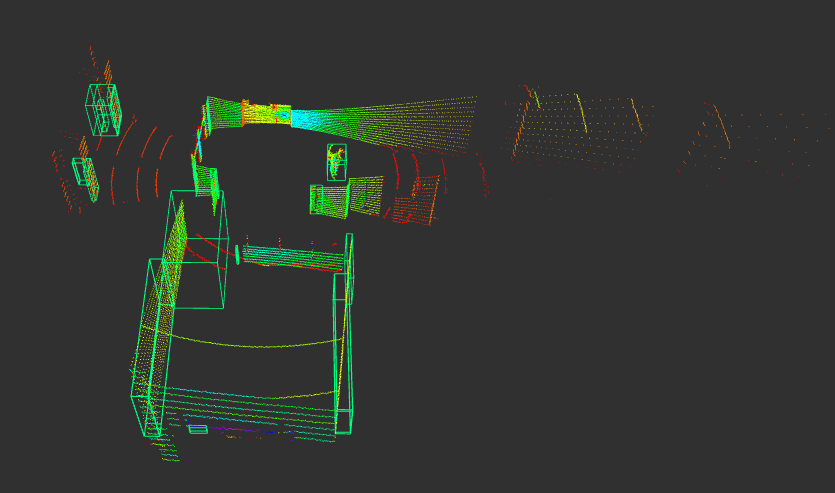
\includegraphics[width=1.0\linewidth,height = 1.0\linewidth]{figures/chap3_fig/onlineSVM/online_train_round1.png}
%     %   \caption{Taking notes with paper \cite{note_paper}}
%       \label{fig:sub1}
%     \end{subfigure}%
%     \begin{subfigure}{.5\linewidth}
%       \centering
%       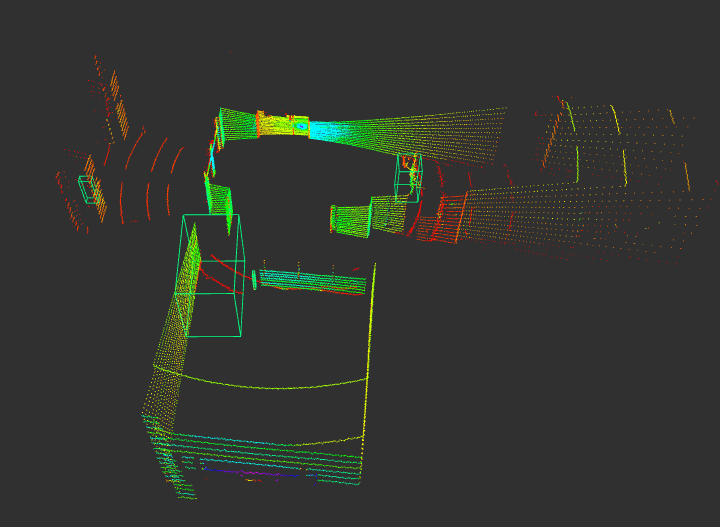
\includegraphics[width=1.0\linewidth,height = 1.0\linewidth]{figures/chap3_fig/onlineSVM/online_train_round3.png}
%     %   \caption{Taking notes with Ipad \cite{note_ipad}}
%       \label{fig:sub2}
%     \end{subfigure}
%     \caption{Icart-mini robot with Velodyne VLP-16}
%     \label{Fig2}
% \end{figure}


\newpage

%------------3.2.4--------------------------------------%
\subsection{PID for Robot controller}
\label{pid_section}

The online learning stage above will yield human cluster's centered position and this data
will be used as input for the PID controller. To successfully follow a human, errors between the
state of robot and human must be diminished to the fullest extent. In actual experiment, z-coordinate of
both human and robot is not essential for the following step. We will only consider offset angle and distance
between the robot and human \cite{refchap2-fig1,DL_Color_feature}, as illustrated in Figure \ref{Chap3:Fig20}.

\begin{figure}[h]
    \centering
    \hspace*{2cm}
    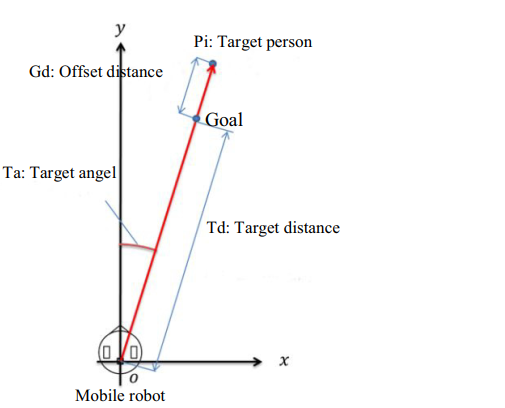
\includegraphics[scale=0.8]{figures/chap3_fig/pid/pid_framework_2.png}
    \caption{Human target distance and direction of mobile robot \cite{hfr_lrs}}
    \label{Chap3:Fig20}
\end{figure}

General offset angle and distance can be determined as in Equation \ref{Chap3:Eq3}. It is
worth noting out that in our case, output human cluster's position is with respect to
the LiDAR sensor's reference frame. In section \ref{Experiments_design_subsection}, one will see that LiDAR and
mobile robot is designed to have same z-axis and same x and y direction. Thus, in 2D format, sensor's frame
coincides with robot's frame and $x_r$ and $y_r$ can be set to zero for simplicity. This equation can
also be used in global coordinate map with tf library \cite{tf_lib} in ROS.

\begin{equation}
    \label{Chap3:Eq3}
    \begin{split}
        d = \quad & \sqrt{(x_h - x_r)^2 + (y_h - y_r)^2} \\
        \theta =  \quad & \taninv {\frac{y_h - y_r}{x_h - x_r}}
    \end{split}
\end{equation}

\newpage

For the following state, PID equation can be used as follows:


% \begin{equation} \renewcommand{\arraystretch}{1.8}
%     \label{Chap3:Eq3}
%     \begin{pmatrix}
%         \dot{x}(t) \\ \dot{y} (t) \\ \dot{z} (t)
%     \end{pmatrix}= K_p \begin{pmatrix}
%         e_x (t) \\e_y (t)\\e_z (t)
%     \end{pmatrix} + K_i \int_{0}^{T} \begin{pmatrix}
%         e_x (t) \\e_y (t)\\e_z (t)
%     \end{pmatrix} \mathrm{dt} + K_d \frac{d}{\mathrm{dt}} \begin{pmatrix}
%         e_x (t) \\e_y (t)\\e_z (t)
%     \end{pmatrix}
% \end{equation}

\begin{equation} \renewcommand{\arraystretch}{1.8}
    \label{Chap3:Eq4}
    \begin{pmatrix}
        v_t \\ \omega_{t}
    \end{pmatrix}=
    \begin{pmatrix}
        \dot{d}(t) \\ \dot{\theta} (t)
    \end{pmatrix}= K_p \begin{pmatrix}
        e_d (t) \\e_{\theta} (t)
    \end{pmatrix} + K_i \int_{0}^{T} \begin{pmatrix}
        e_d (t) \\e_{\theta} (t)
    \end{pmatrix} \mathrm{dt} + K_d \frac{d}{\mathrm{dt}} \begin{pmatrix}
        e_d (t) \\e_{\theta} (t)
    \end{pmatrix}
\end{equation}

with distance error $e_d = (d - D)$ and angle error $e_{\theta} = \theta - \Theta$. They can
also be called as state differences , where $D$ and $\Theta$ are target distance and angle respectively.
In this following step, $D$ is set to be 1m and $\Theta$ is around $5^o$. 3 PID parameters $K_p$ , $K_i$ and $K_d$
are set differently for each testing environment, namely corridor and testing hall (See Chapter \ref{Chap:ExperimentSetup_Results}). These values
are tuned by trial and error until reliable result is attained.

However,to ensure the robot follows the exact
initial person, the position of the human between 2 consecutive detections will be constrained to be no larger
than a maximum distance. We denote $r_t$ as the distance between 2 consecutive recognition and human-filter based velocity is set
as follows:

\begin{equation}
    \label{Chap3:Eq5}
    \begin{split}
        r_t = \quad & \sqrt{({x_h}^t - {x_h}^{t-1})^2 + ({y_h}^t - {y_h}^{t-1})^2} \\
        r_t \leq  \quad &  {v_h}^{max} \Delta t
    \end{split}
\end{equation}

After setting constraints as in Equation \ref{Chap3:Eq5}, target goal or target human's position is fed to the PID
feedback loop as in Equation \ref{Chap3:Eq4} above. This completes the whole process of the proposed pipeline. Final pipeline
result is presented in section \ref{pipeline_result}.